\section{Task 8 at SemEval 2024}
\label{sec:task}

The 18th International Workshop on Semantic Evaluation (SemEval-2024) was a large event in NLP, offering various challenges that teams across the world could undertake.
Task 8 at SemEval-2024 \citep{wang2024semeval} centered around machine-generated text detection in a black-box setting (i.e., the generator models for the test set were not known while the competition was ongoing), in both monolingual and multilingual components.

This shared task spanned 3 subtasks: subtask A a binary classification task between generated and human texts, subtask B consisted in multi-class classification between multiple LLM generators, as well human texts, while subtask C was a boundary detection problem, where participants had to correctly pinpoint the boundary between a human and a machine-generated segment in each test.
During the active phase of SemEval-2024, which ended in February 2024, I undertook Task 8 jointly with Daniel Stuhlinger, a fellow student at the University of Tübingen.
The full report of our participation, carried out under the team name "TueCICL", can be viewed in \citet{stuhlinger-winkler-2024-tuecicl}.

As team TueCICL, we submitted results for two of the subtasks to the leaderboards, namely subtask A and subtask C, which were the two subtasks involving classification between solely human and machine-generated texts, whereas subtask B focused more on inter-generator differentiation.
For subtask A, consisting in binary classification over the whole texts, there were two phases development, one for shared task proper, and subsequent post-deadline experimenting in the context of this Master Thesis.
Due to the more pronounced research interest in subtask A, as well as to better present the higher volume of material associated with it, this section shall first discuss subtask C, then dive deeper into subtask A later in this Chapter.

\subsection{Human - LM Boundary detection}

Subtask C of the shared task addresses detection environments that are characterized by active adversarial agents performing the generation.
Specifically, detection technologies have been observed to be weak to techniques also found in obfuscation \citep{macko2024authorship}, such as paraphrasing \citep{krishna2024paraphrasing} and noise-introduction \citep{wang2021adversarial}.
Change point detection, which is the titular requirement of subtask C, addresses another way in which the use of NLG technology might be obfuscated.
In the scenario targeted by the subtask, a human segment ranging from 0\% to 50\% of the text is concluded by a machine-generated component, making the text as a whole much harder to flag as a generation.

Task organizers provided generations by GPT variants and the LLaMA series \citep{touvron2023llama}, but unfortunately not in high abundance: the training set around 5000 texts, and was accompanied by development set containing a little over 500 more.
Table \ref{fig:taskc_data} offers an overview of the data distribution across the sets.


\begin{figure}[h]
    \centering
    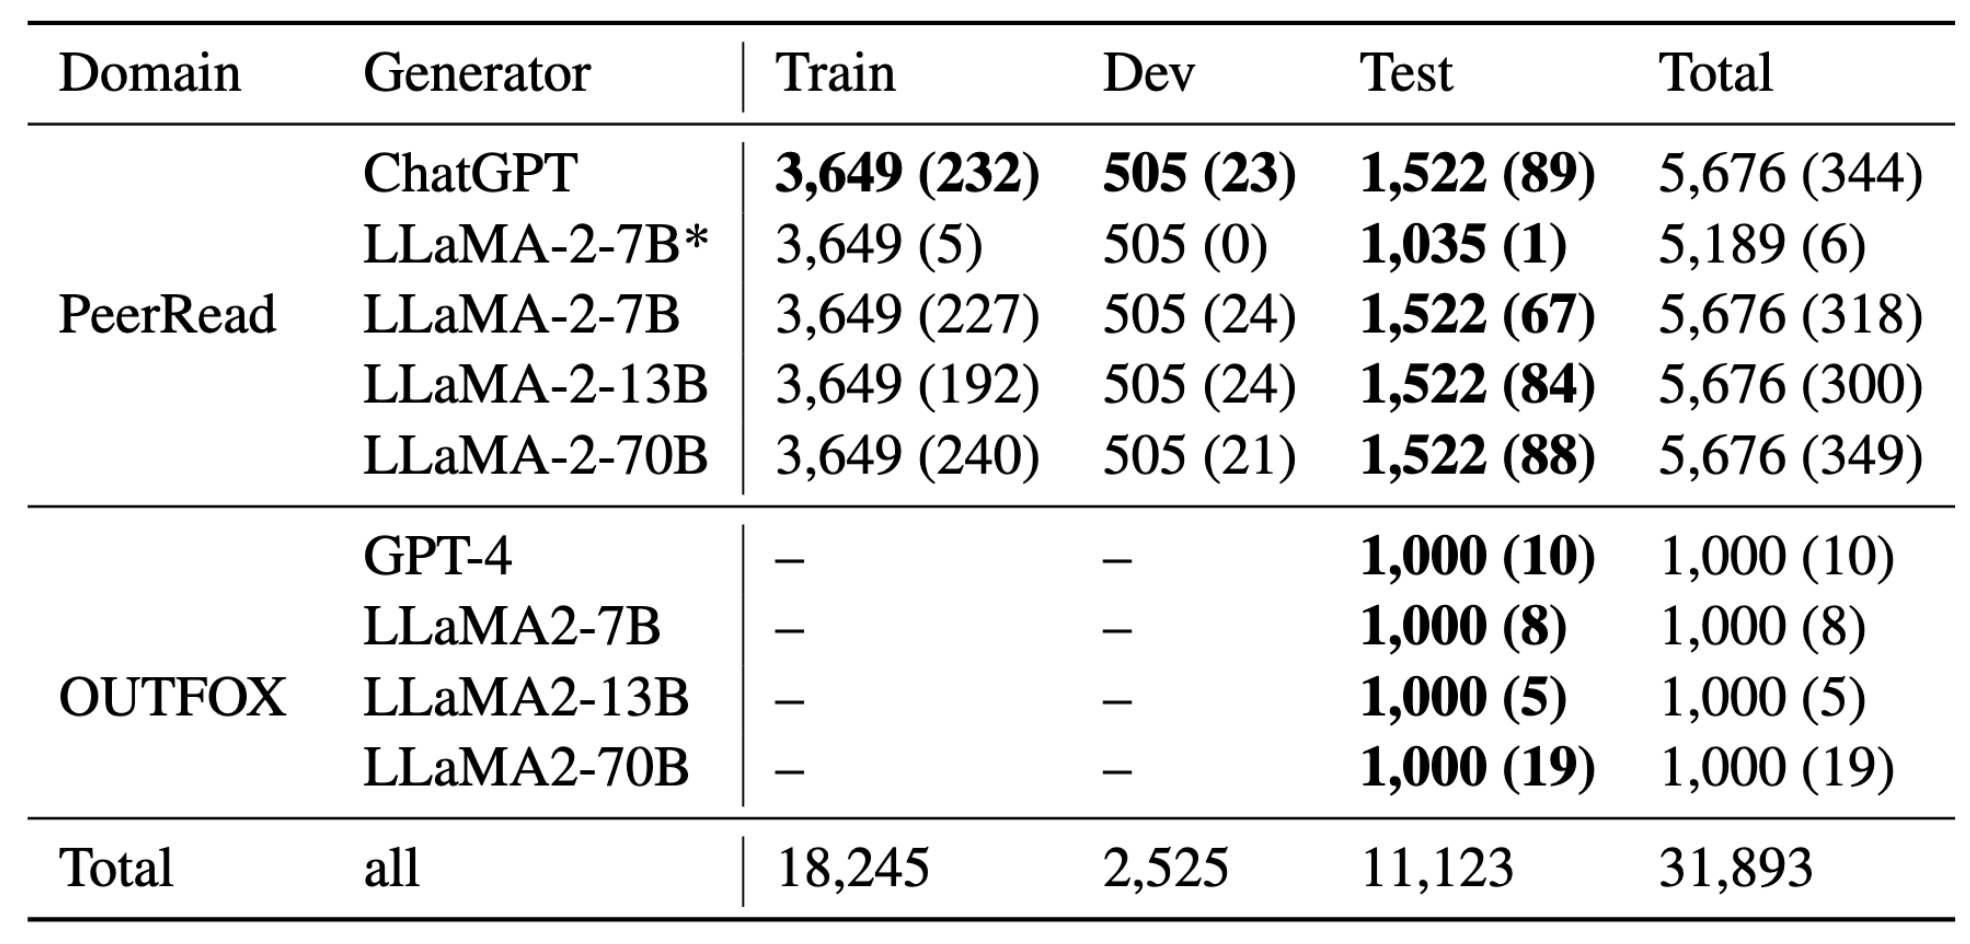
\includegraphics[width=0.5\textwidth]{assets/subtaskc-data.png}
    \caption{
        Dataset breakdown for subtask C from Task 8 at SemEval-2024.
        The number in “()” is the number of examples purely generated by LLMs, i.e., human and machine boundary index=0.
        LLaMA-2-7B* and LLaMA-2-7B used different prompts. Bold data is used in shared task training development, and test.
    }
    \label{fig:taskc_data}
\end{figure}

\subsection{Generated text detection}
\label{subsec:subtask_a}

\subsection{Generated text detection: post-deadline additions}